\section{Used Models}
\label{sec:used_models}


This section provides an extensive description of the models used in our experiments. We focused on three main types of models: point cloud-based models, transformer-based models, and persistence-based models. Since the latter require background on persistence homology, they're further detailed in Section~\ref{ssec:ph}. On the one hand, point cloud-based models are used as baselines for specific tasks (see Table~\ref{tab:topogen-results}). This choice stems from the widely known limitations in terms of robustness to input corruption and generalization~\cite{set-transformer} of such models. On the other hand, transformers have demonstrated state-of-the-art performance on various 3D shape understanding tasks~\cite{pbert,pmae,pm2ae,pcpmae}, and we are therefore insterested here in their ability to learn rich representations from data.

\subsection{Baselines Models}
\label{ssec:baselines_models}

We compare results obtained with transformer-based models to several baselines widely used in the literature. These models directly act on individual points without any tokenization step. They are all invariant to point permutations and can handle varying point cloud sizes. A final feature vector is obtained through a global pooling operation, which is then used for downstream tasks.

\subsubsection{PointNet}

PointNet~\cite{pointnet} introduced the first deep learning architecture that operates directly on raw 3D points. Each point is independently transformed through shared multilayer perceptrons (MLPs) to extract per-point features, which are then aggregated using a symmetric pooling function—typically max pooling—to obtain a global shape descriptor. This design ensures invariance to input permutation and robustness to geometric transformations through a learned spatial transformer network. However, since PointNet treats each point independently before pooling, it lacks the ability to explicitly capture local geometric structures and neighborhood relations within the point cloud.

\subsubsection{PointNet++}

PointNet++~\cite{pointnet++} extends PointNet by introducing a hierarchical feature learning mechanism that captures local geometric patterns at multiple scales. It partitions the point cloud into overlapping local regions using sampling and grouping operations, applies PointNet within each region to extract local features, and recursively aggregates them to form higher-level representations. This hierarchical structure allows PointNet++ to model fine-grained local geometry while maintaining the permutation invariance of PointNet. The introduction of radius-based grouping and multi-scale feature extraction significantly improves robustness to non-uniform sampling and enhances generalization to complex shapes.

\subsubsection{DGCNN (Dynamic Graph CNN)}

DGCNN~\cite{dgcnn} further advances local structure modeling by representing the point cloud as a dynamic graph, where edges connect each point to its k-nearest neighbors in the feature space. Unlike PointNet++’s static grouping, DGCNN updates the neighborhood graph at each layer, allowing feature dependencies to evolve adaptively as the representation becomes more abstract. The model applies an edge convolution operator that learns features based on both point attributes and relative positional differences, effectively capturing local geometric relations and contextual information. This dynamic graph formulation enables DGCNN to achieve strong performance on tasks requiring fine spatial reasoning, such as segmentation and shape classification.

\subsection{Transformer-based models}
\label{ssec:transformer_based_models}

\begin{figure}[t]
  \centering
  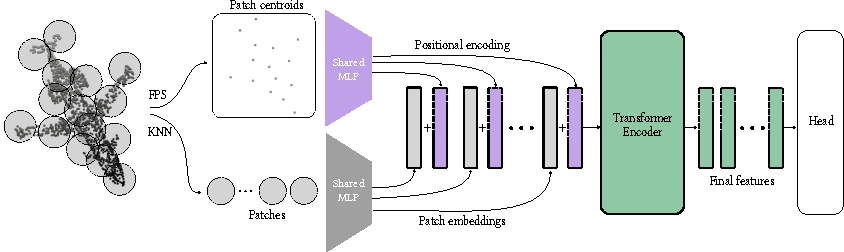
\includegraphics[width=1.0\linewidth]{figs/transformer_overview.pdf}
   \caption{\textbf{Transformer Overview for 3D point-clouds.} A point cloud is first partitioned into local patches using farthest point sampling (FPS) and K nearest neighbors (KNN). Patches are then embedded and augmented with positional encodings. The resulting sequence of patch embeddings is processed by a Transformer encoder to produce a global shape representation.}
   \label{fig:transformer-overview}
\end{figure}

Recent advances in transformer architectures for 3D shape understanding have largely built on the intuition that ideas from NLP and vision can be transferred to point cloud data. While the geometry of 3D shapes is fundamentally different from text or images, most models share a similar pipeline. A point cloud is first partitioned into a set of local patches. This is commonly achieved with farthest point sampling, and then grouping each center with its nearest neighbors to form a subcloud. Each of these patches is then embedded into a high-dimensional space using a lightweight encoder, typically a variant of PointNet or DGCNN that aggregates local geometric features while maintaining permutation invariance.

To preserve spatial structure, positional encodings are added by projecting the coordinates of the patch centers through an MLP, which provides the transformer with a notion of relative geometry between patches. The resulting sequence of patch embeddings, optionally augmented with a learnable global "class token" is then fed into a Transformer encoder. This process is conceptually identical to Vision Transformers, where image patches are tokenized, embedded, and processed sequentially, though here the tokens correspond to irregular geometric neighborhoods rather than regular image patches.

This generic framework has provided the foundation for several influential works that differ primarily in how tokens are defined, how self-supervised pretraining is formulated, and whether hierarchical representations are incorporated. We now discuss these paradigms in detail.

\subsubsection{Point-BERT: Discrete Tokenization and Masked Modeling}
\label{sssec:pointbert}

One of the earliest attempts to port the BERT paradigm to point clouds is Point-BERT \cite{pbert}. Its central idea is to treat a point cloud as a sequence of discrete tokens, thereby enabling the use of masked language modeling (MLM) for self-supervised pretraining. To achieve this, Point-BERT first trains a discrete variational autoencoder (dVAE) to learn a vocabulary of geometric tokens. The encoder of the dVAE maps continuous patch embeddings into discrete codewords, while the decoder reconstructs the original patch from the codeword, ensuring that the learned vocabulary captures meaningful local geometry.

With this vocabulary in place, Point-BERT pretrains the Transformer using Masked Point Modeling (MPM): a subset of input patches are masked, and the model is trained to predict the corresponding discrete token indices assigned by the dVAE. This formulation parallels masked language modeling in NLP, where the model predicts missing words from context, but here the "words" are geometric patches. Importantly, Point-BERT also incorporates a learnable class token that is updated jointly with the patch tokens during pretraining. The final embedding of this class token is then used for downstream classification and retrieval tasks, mirroring the global semantics captured by the CLS token in NLP transformers.

This approach makes pretraining strongly analogous to BERT, but it requires a two-stage pipeline, first learning the tokenizer and then training the transformer, which introduces additional complexity. Nonetheless, Point-BERT demonstrated that masked token prediction is a powerful way to learn shape priors from unlabeled point clouds.

\subsubsection{Point-MAE: Continuous Tokens and Masked Autoencoding}

While Point-BERT relies on discrete tokenization, Point-MAE~\cite{pmae} instead follows the Masked Autoencoder (MAE)~\cite{mae} framework introduced in vision. Here, patches are represented by continuous embeddings rather than discrete vocabulary entries, and the pretraining task is reconstruction rather than classification. Specifically, Point-MAE applies a high masking ratio (often exceeding 60\%) to the input patches. Only the unmasked patches are fed through the heavy transformer encoder. Masked patches are replaced with a shared mask token, and both unmasked embeddings and mask tokens are processed by a lightweight decoder tasked with reconstructing the original 3D coordinates of the masked patches.

This approach has several advantages. First, it avoids the need for a separate tokenizer, simplifying the training pipeline. Second, it is more computationally efficient: since the encoder processes only unmasked patches, the model scales better to large point clouds. Third, it allows the model to directly learn continuous geometric representations, which are more flexible than a finite vocabulary.

Unlike Point-BERT, Point-MAE does not include a CLS token during pretraining. Instead, the class token is introduced only when the model is fine-tuned on downstream tasks. This choice emphasizes that the focus of pretraining is purely local reconstruction, while global semantics can be learned in task-specific adaptation. Overall, Point-MAE demonstrated that masked autoencoding provides a simple yet effective way to pretrain 3D transformers, establishing a new standard for self-supervised learning on point clouds.

\subsubsection{Hierarchical Extensions: Multi-Scale Representations}
\label{sssec:hierarchical_extensions}

A third line of work emphasizes that 3D shapes are inherently hierarchical, with geometric structures manifesting at multiple scales. This insight parallels the evolution from PointNet to PointNet++, where hierarchical feature extraction proved essential for robust representation learning. 

Point-M2AE~\cite{pm2ae} extends Point-MAE by introducing a multi-scale transformer architecture. The encoder progressively downsamples the point cloud into coarser patches, capturing increasingly global features, while the decoder reconstructs masked patches using skip connections, reminiscent of U-Net architectures. In addition, Point-M2AE employs a multi-scale masking strategy to ensure consistency across levels of abstraction and introduces local spatial self-attention at fine scales to better capture detailed geometry. This design not only improves parameter efficiency but also strengthens the model’s ability to capture structures across varying spatial resolutions.

\subsubsection{Further Improvements}
\label{sssec:further_improvements}

Most recent approaches have mainly built on top of Point-MAE, primarily for the training setting, easier than Point-BERT. PCP-MAE~\cite{pcpmae} modifies positional encoding to prevent information leakage: instead of directly using patch centers, which can trivially reveal masked locations, it requires the model to predict them. HFBRI-MAE~\cite{hfbrimae} incorporates handcrafted rotation-invariant features as both tokens and positional encodings, improving robustness under arbitrary 3D rotations. Point-RAE~\cite{prae} proposes a regression-before-autoencoding strategy to decouple encoder and decoder representations, thereby avoiding the risk of the decoder dominating feature learning. Collectively, these hierarchical and refined models show that injecting geometric inductive biases into the transformer architecture can significantly improve generalization and robustness.

\subsubsection{Comparative View}
\label{sssec:comparative_view}

Despite their differences, Point-BERT, Point-MAE, and their hierarchical successors share a common foundation: the adaptation of the transformer paradigm from language and vision to point clouds through \textit{patchification}, embedding, and positional encoding. What distinguishes them is how tokens are defined, how the self-supervised objective is formulated, and whether hierarchical geometry is explicitly modeled. Discrete-token approaches like Point-BERT require a two-stage pretraining pipeline but tightly align with NLP pretraining paradigms. Continuous-token methods like Point-MAE are simpler and more efficient, emphasizing reconstruction over classification. Hierarchical extensions such as Point-M2AE incorporate multiscale representations, bringing additional inductive structure into the transformer.

An important consequence of these differences is that evaluation protocols vary across models. Point-BERT pretraining relies on predicting discrete token IDs, while Point-MAE and M2AE use reconstruction losses such as Chamfer distance. The role of the CLS token also differs, being central during pretraining in Point-BERT but absent in MAE-style approaches. As a result, downstream fine-tuning and linear probing must be carefully adapted to each architecture. The precise evaluation settings for each method will be detailed in the following experimental section.